% !TeX root = ../main.tex

\chapter{水下穿戴式感知增强系统设计}
潜水员在水下复杂环境中进行作业任务时对周围环境感知能力有限,为了帮助潜水员在水下作业时提供全面的外界感知,
本章基于前面章节所提出的水下图像增强算法和三维重建技术设计了一种可穿戴式的水下感知增强系统。
首先结合实际应用场景进行需求分析和可行性分析,从实用性角度系统讨论了平台架构和功能设计要点。
系统通过将水下图像增强算法和三维重建技术集成到可穿戴式头显中并结合手势识别技术作为交互手段,
方便潜水员在恶劣的水下环境中获取更加全面和清晰的水下环境信息,从而提升潜水员在诸如检修、勘探等水下作业时的作业效率。

\section{需求分析和可行性分析}

需求分析和可行性分析是系统设计过程中至关重要的步骤。需求分析的作用在于明确系统的功能和性能要求,确保系统能够满足用户的实际需求。
通过对潜水员在水下作业时的具体需求进行详细分析,可以为系统的设计提供明确的方向和目标。
可行性分析则是在需求分析的基础上,对系统设计方案具体实现方式进行讨论,确保系统的设计方案在满足需求的前提下,具有可实现性。
通过需求分析和可行性分析,可以有效降低系统设计的风险,提高系统的可靠性。

\subsection{需求分析}
针对潜水员在水下复杂环境中的感知受限问题,本系统以提升潜水员的环境感知能力为核心目标,
主要从改善水下视觉图像和提供水下三维场景预览两个角度,
构建基于水下图像增强技术与三维重建技术的具备辅助感知增强的可穿戴系统。
结合实际应用场景,具体需求可以分为以下四个方面:

(1)水下视觉增强:通过集成先进的水下图像增强算法和三维重建技术,系统应当能够在水下环境中提供高质量的视觉信息,
这不仅包括清晰的图像和视频,还包括逼真的三维场景渲染,
帮助潜水员随时预览水下作业环境,以帮助潜水员在视野受阻的复杂水下环境中更好地掌握周围环境信息,
从而提升潜水员在诸如检修、勘探等水下作业时的作业效率。

(2)实时三维渲染:本系统以虚拟现实技术为载体,借助 3D 高斯泼溅技术为潜水员提供水下场景的全视角三维渲染图预览。
潜水员需依赖头戴式显示器来获取水下作业环境信息,
为了确保潜水员能够流畅的实时阅读周围环境信息,系统在进行三维图像渲染时应当确保渲染速率不低于30fps。

(3)可靠的运行平台:水下环境的特殊性给系统的结构设计带来了极高的要求,
系统的所有组件,包括头戴式显示器和搭载嵌入式计算单元的水下背包,需要具备良好的密闭性和防水性,
以在水下高压和腐蚀性环境中可以保持稳定运行。

(4)自然的人机交互:人机交互是穿戴式设备的重要组成部分,水下穿戴式设备应当避免使用过多传统的物理按键,防止平台对外暴露过多的物理接口,
系统需要以一种更加方便直观的人机交互方式,为潜水员与系统之间提供自然的人机交互。

\subsection{可行性分析}
从视觉增强功能完整性和系统实时性角度来说,根据第三章水下图像增强算法具体介绍以及实验结果可以看出,
该算法可以有效提升水下原始图像的质量,更重要的是其具备恢复图像的语义信息的能力,这为后期基于特征匹配的SfM点云生成具有可行性。
虽然该算法在实时性方面表现较差,但本系统对图像增强的功能定位是为后续的 3D 高斯泼溅算法提供高质量的水下图像输入,所以系统对该算法在实时性方面的要求不高。
另外,第四章提出的基于 3D 高斯泼溅的水下三维重建算法,继承了原始 3DGS 方法的实时渲染能力,同时本系统在硬件平台上也可以选择具有高性能边缘计算能力的嵌入式处理器,
以确保系统能够为潜水员提供高帧率的全视角场景图像,提升系统使用体验。

从系统可靠性角度来说,本系统的设计难点在于如何保证整体结构在水下保持良好的密封性,
其中头戴式显示器、相机、嵌入式处理器等组件可以通过使用防水材料(涂料)和密封结构设计使其能够在水下高压和腐蚀性环境中保持稳定运行。
另外,相关组件之间也可以尽量采用更加一体化的设计方案,减少暴露过多的连接接口。

从人机交互角度来说,本系统的交互需求主要体现在如何让潜水员在水下可以更加便捷的与三维场景预览界面进行交互。
基于现有的水下手势识别算法,本系统可以通过建立一套直观而有意义的手势指令,为潜水员提供更加直观且自然的人机交互,
这种基于手势识别的交互方式可以减少大量的实体物理按键,防止过多物理按键给防水带来额外的难度,
同时也可以有效避免物理按键在防水结构下的操作不便问题,提升潜水员在三维场景中的沉浸感。

如上所述,本系统在功能、实时性、可靠性和交互性上均具备可行性,在潜水员进行水下作业时可以作为一种有效的辅助感知增强手段。

\section{系统平台搭建} 
\subsection{硬件选型与系统架构}
结合对系统的需求分析和可行性分析,系统核心功能主要通过首先获取水下场景图像,再利用算法增强图像质量,把增强后的图像作为训练数据优化水下三维建模,
然后基于训练好的三维模型在嵌入式设备上进行实时渲染,最后借助头戴式显示器将渲染结果反馈给潜水员,以实现水下感知增强的目的。
因此该水下穿戴式感知增强系统主要是由相机、头戴式显示器、嵌入式处理器以及电源模块等必要组件所构成。

(1)相机:
系统选用两个相同型号的 RGB 相机作为主摄,可以拍摄分辨率为1920x1080,帧率为90fps的RGB图像,系统利用这两组图像来模拟人双眼看到的画面,
两个主摄相机通过透明亚克力面板封装在由聚丙烯材料3D打印的外壳内,保证其在水下高压环境中的稳定性。

(2)头戴式显示器:
头显采用 5 英寸显示屏,分辨率为 1920x1080 像素,与相机分辨率一致,确保潜水员可以清晰地查看相机捕获的图像和预览三维模型渲染的画面。
显示器通过微型 HDMI 与嵌入式处理器连接,外壳基于谷歌 VR 纸板设计并用聚丙烯材料3D打印,同时用环氧树脂进一步做了防水处理,确保水下使用的可靠性。

(3)嵌入式处理器:
系统选用NVIDIA Jetson Orin Nano作为核心计算单元,其具备强大的边缘计算能力,GPU架构为Ampere,拥有48 Tensor Cores,
支持深度学习推理加速,能够实时处理去噪扩散模型和3D高斯泼溅算法所需的计算任务。
处理器支持10W和20W两种功耗模式,结合自适应供电机制,确保系统在高性能和低功耗之间平衡。

(4)电源模块:
系统采用高容量锂电池组,容量为20,000mAh,输出电压为12V,满足Jetson Orin Nano的供电需求。
电池组集成于防水背包中,通过防水接头连接处理器,具备充电和过载保护功能,确保长时间潜水作业的稳定运行。

如图\ref{img:system}所示,相机与显示屏一体化封装在头戴式外壳内,电源模块和嵌入式处理器集成在 3D 打印的防水背包中,
头戴式设备和背包之间的数据与供电传输线缆通过防水接头连接,并采用环氧树酯AB胶水对接头进行灌装密封处理,确保系统在水下高压和腐蚀性环境中保持稳定运行。
背包通过穿戴式马甲背带固定在潜水员背部,同时提供魔术贴来调整背包的穿戴高度与松紧度,不同使用者可以按照自身体型进行合适的调整,以确保潜水员在潜水过程中能够舒适地穿戴该系统。

\begin{figure}
    \vspace{4mm}
    \centering
    \includegraphics[width=0.85\textwidth]{figures/ch5/system.pdf}
    \caption{水下穿戴式感知增强系统组成}
    \label{img:system}
\end{figure}

\subsection{防水与机械设计}
在水下环境中,设备的防水性和密封性是决定系统可靠性的重要因素,
本系统对头戴式设备和背包的进行了充分的防水与密封设计,以确保系统在水下环境中保持稳定运行。

(1)防水背包:
\begin{figure}[h]
    \centering
    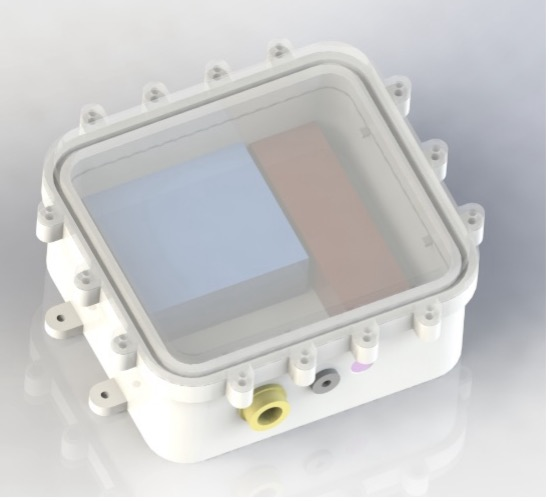
\includegraphics[width=0.5\textwidth]{figures/ch5/bag.jpg}
    \caption{防水背包结构}
    \label{img:bag}
\end{figure}

如图\ref{img:bag}所示,背包外壳采用高强度工程塑料,表面涂覆防水涂料做防水处理。
密封方式采用多层硅胶垫片与不锈钢紧固件结合,确保防水等级达到IP68。
出线采用专用防水接头和穿线螺丝,接口部分环氧树脂AB胶水灌装密封,进一步增强防水性能。
为了实现浮力与重力平衡,系统还在背包底部嵌入两块承重铁块,实现系统在水下的“零浮力”。

(2)头戴式显示设备:
\begin{figure}[h]
    \vspace{1mm}
    \centering
    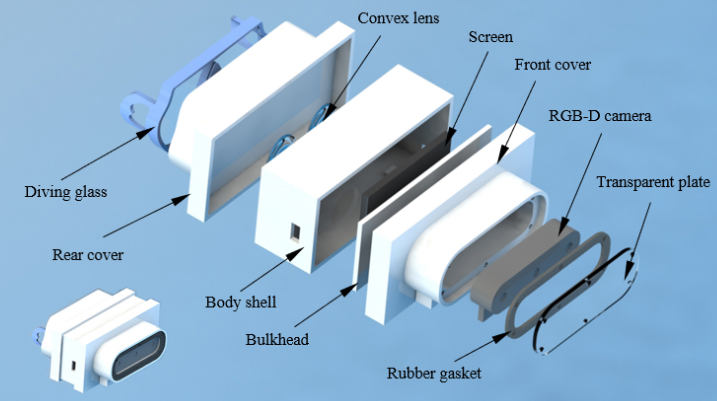
\includegraphics[width=0.85\textwidth]{figures/ch5/headscreen.pdf}
    \caption{头戴式显示设备结构}
    \label{img:camera}
\end{figure}

如图\ref{img:camera}所示,
配有双RGB主摄的相机安装于头显前端,相机正面用透明亚克力外壳封装于头显主体之中,
头显主要通过3D聚丙烯材料打印制作,与背包一样在表面涂覆防水涂料做防水处理,
外壳面板之间通过橡胶圈进行紧密的密封连接,确保在水压变化下不发生渗漏。
头显的观察凸透镜片采用聚碳酸酯材料,经过耐冲击和防刮擦处理。
镜框与镜片之间采用液态硅胶封装,并在边缘增加防护垫圈。
最后,利用潜水眼镜面罩将头显与潜水员面部紧密贴合,确保头显在潜水过程中不会脱落。

另外,各部件之间的线缆通过防水接头连接,并用环氧树酯AB胶水对接头进一步灌装密封处理,如图\ref{img:cable}所示。
\begin{figure}
    \vspace{4mm}
    \centering
    \includegraphics[width=0.6\textwidth]{figures/ch5/cable.pdf} \hspace{-3.5cm}
    \caption{线缆连接}
    \label{img:cable}
\end{figure}

\section{整体功能设计}
本章设计的水下感知系统主要由嵌入了防水背包的防水背包以及头戴式显示设备组成,
该系统能够将直接捕捉的视觉数据反馈至头戴式显示设备,
并通过 Jeston Orin 处理器实时渲染提前处理好的水下三维场景,
结合手势识别技术对三维预览界面进行视角控制,实现在水下的感知增强。

\subsection{图像增强与三维重建}
本文提出的水下可穿戴感知增强系统,通过整合第三章提出的水下图像增强算法和第四章的三维重建技术,目的在于为潜水员提供高质量和逼真的水下三维场景。
系统整体功能设计如图 \ref{img:function} 所示,包含从数据采集到模型部署的全流程设计方案。
\begin{figure}[ht]
    \centering
    \vspace{0.5cm}
    \includegraphics[width=0.97\textwidth]{figures/ch5/function.pdf}
    \caption{系统功能设计}
    \label{img:function}
\end{figure}

系统首先需要采集目标水下场景的多视角图像数据为三维重建做准备,为了确保采集的全面性和灵活性,可以利用AUV或ROV围绕目标区域进行多视角的视频拍摄。
对于采集到的视频数据,采用抽帧方法获取带有时序信息连续的图像序列,然而,受制于水下环境的特性(如光散射、颜色失真、低对比度等),原始水下图像通常存在模糊、色偏和细节丢失问题,这为后续的特征点匹配和点云生成带来了显著挑战。
为解决这些问题,系统集成了第三章介绍的基于去噪扩散模型的水下图像增强算法。该算法能够有效修复水下图像视觉特征,生成语义信息丰富且高感知质量的水下图像,为后续的三维重建提供了更为可靠的数据基础。

然后,系统将利用SfM框架流程进一步处理图像数据,完成初步的点云生成与相机位姿估计。
SfM 技术的核心优势在于,即便在无相机内部参数的情况下,也能通过 2D 图像之间的特征点匹配,推断出相机的位姿以及场景的初步三维点云数据。
系统将处理好的水下图像输入 SfM 算法,通过精确的特征点匹配生成初始三维点云数据及对应的相机位姿。
这些点云数据往往较为稀疏,难以直接支持高质量三维模型的构建。
为此,系统引入基于算法 \ref{eq:knn} 的点云补充策略,通过近邻搜索对稀疏点云进行插值与补全,生成更为稠密的点云数据。
这一过程为后续的三维高斯模型训练提供了丰富的数据支撑,可以避免在初始化训练阶段因数据不足导致的不稳定性。

在点云数据准备充分的情况下,系统利用第四章介绍的基于 3D 高斯泼溅的三维重建算法完成水下场景的多训练过程。
训练也可以在地面端进行,通过高性能计算设备对三维模型进行迭代优化,以确保模型能够精确还原水下场景的细节与结构。
训练好的三维模型可以部署到轻量级的嵌入式设备 Jetson Orin Nano 中,实现任意视角画面的渲染,以反馈给潜水员进行实时预览。

\subsection{用户交互与控制}
水下穿戴式感知系统需要考虑潜水员在水下环境中的操作便利性,而对于三维场景的预览往往需要多种按键的配合使用才能实现全方位的视角控制,
如图\ref{img:gaussianviewer}所示,SIBR Gaussian Viewer 软件支持FPS第一人称导航视角控制方式来对训练好的 3D 高斯模型的渲染结果进行浏览,
其需要六个移动按键来控制视角的上下左右和前后方向的移动以及六个旋转键位来控制对应的旋转,在某些情况下潜水员需要频繁的进行视角的调整才能找到目标视角,这给水下作业带来了极大的操作不便。
此外,在原有平台上提供多个物理按键给潜水员使用需要增加额外的操控模块,这会增加机械结构设计的复杂度,多出的操控模块也会影响原有的系统集成性,增加系统整体的防水难度。
\begin{figure}[ht]
    \centering
    \vspace{0,4cm}
    \includegraphics[width=0.98\textwidth]{figures/ch5/viewers.png}
    \caption{SIBR Gaussian Viewer 软件界面}
    \label{img:gaussianviewer}
\end{figure}

RoboChatGest\cite{robochatgest}是一种专门为潜水员和水下机器人进行协作交互所设计的手势识别算法,其结合深度视觉感知器获取潜水员的手势信息,并利用预训练的神经网络模型进行准确的手势识别,
潜水员可以使用一套直观而有意义的手势与机器人进行交互。受 RoboChatGest 的启发,为了提高潜水员在水下环境中的操作便利性,本文为提出的水下穿戴式感知增强系统设计了一套基于手势识别的用户交互方案,潜水员可以通过设定的手势指令完成与三维可视化场景预览界面的交互。

结合水下穿戴式感知系统的交互需求,本文选取了 RoboChatGest 中的一个视觉上更独特和直观的小手势集作为最后的交互手势原语,如表\ref{tab:chatgest}所示。

\begin{table}
\vspace{0.1cm}
\caption{手势识别原语}
\centering
\begin{tabular}{|c|c|c|c|c|c|c|c|c|c|}
\hline
\textbf{0} & \textbf{1} & \textbf{2} & \textbf{3} & \textbf{4} & \textbf{5} & \textbf{left} & \textbf{right} & \textbf{pic} & \textbf{ok} \\ \hline
\adjustbox{valign=c}{\includegraphics[width=1cm]{figures/ch5/res/d0.jpg}} & 
\adjustbox{valign=c}{\includegraphics[width=1cm]{figures/ch5/res/d1.jpg}} & 
\adjustbox{valign=c}{\includegraphics[width=1cm]{figures/ch5/res/d2.jpg}} & 
\adjustbox{valign=c}{\includegraphics[width=1cm]{figures/ch5/res/d3.jpg}} & 
\adjustbox{valign=c}{\includegraphics[width=1cm]{figures/ch5/res/d4.jpg}} & 
\adjustbox{valign=c}{\includegraphics[width=1cm]{figures/ch5/res/d5.jpg}} & 
\adjustbox{valign=c}{\includegraphics[width=1cm]{figures/ch5/res/d6.jpg}} & 
\adjustbox{valign=c}{\includegraphics[width=1cm]{figures/ch5/res/d7.jpg}} & 
\adjustbox{valign=c}{\includegraphics[width=1cm]{figures/ch5/res/d8.jpg}} & 
\adjustbox{valign=c}{\includegraphics[width=1cm]{figures/ch5/res/d9.jpg}} \\ \hline
\adjustbox{valign=c}{\includegraphics[width=1cm]{figures/ch5/res/u0.jpg}} & 
\adjustbox{valign=c}{\includegraphics[width=1cm]{figures/ch5/res/u1.jpg}} & 
\adjustbox{valign=c}{\includegraphics[width=1cm]{figures/ch5/res/u2.jpg}} & 
\adjustbox{valign=c}{\includegraphics[width=1cm]{figures/ch5/res/u3.jpg}} & 
\adjustbox{valign=c}{\includegraphics[width=1cm]{figures/ch5/res/u4.jpg}} & 
\adjustbox{valign=c}{\includegraphics[width=1cm]{figures/ch5/res/u5.jpg}} & 
\adjustbox{valign=c}{\includegraphics[width=1cm]{figures/ch5/res/u6.jpg}} & 
\adjustbox{valign=c}{\includegraphics[width=1cm]{figures/ch5/res/u7.jpg}} & 
\adjustbox{valign=c}{\includegraphics[width=1cm]{figures/ch5/res/u8.jpg}} & 
\adjustbox{valign=c}{\includegraphics[width=1cm]{figures/ch5/res/u9.jpg}} \\ \hline
\end{tabular}
\label{tab:chatgest}
\vspace{0.4cm}
\end{table}
% \begin{figure}
%     \centesu a
%     \includegraphics[width=0.95\textwidth]{figures/ch5/chatgest.jpg}
%     \caption{手势识别原语}
%     \label{img:chatgest}
% \end{figure}

系统交互目标是采用一套简单明了的交互手势来完成对三维场景预览界面的控制,而无需潜水员记住复杂的语言规则。
本文基于表\ref{tab:chatgest}所示的十个手势原语的双手组合序列设计了一套键盘控制按键与手势指令的映射关系,
每个手势直观地与其所传递的命令相关联:

(1)任务切换:用于三维视角调整指令的开启与关闭,
当潜水员需要调整视角到想要的位置时,可以通过“开始/突出预览”指令开启界面的视角控制,此时后续的所有互动手势令牌才会生效,
另外,当潜水员持续保持该手势令牌时,系统会把三维场景的预览图像放大突出显示,从而辅助潜水员观察对应视角的画面细节;
而当潜水员已经找到合适的预览视角时,通过“停止”指令关闭视角控制,后续的手势指令将不再生效。

(2)视角的移动:在开启视角调整后,潜水员可以通过左手的手势令牌 “\{5\}” 与右手的六种手势组合来控制视角在X、Y、Z轴上的移动。

(3)视角的旋转:在开启视角调整后,潜水员可以通过左手的手势令牌 “\{pic\}” 与右手的六种手势组合来控制视角在X、Y、Z轴上的旋转。

所有的交互指令映射关系如表\ref{tab:instruction}所示,基于精心设计的交互手势,潜水员可以很快的掌握三维视角的调整控制。
同时,本系统添加了额外的限制:所有手势令牌必须在连续检测到 5 帧后才会激活,这种约束可以丢弃一些由于手势识别错误或者潜水员切换手势时产生的嘈杂令牌,提高系统的稳定性,
此外,由于映射是一对一的,即使潜水员错误地执行了一些不准确的手势,也很难生成错误的指令,因为每个状态除了正确的映射规则外,没有其他映射规则。
\begin{table}[h!]
\vspace{1mm}
\caption{SIBR Gaussian Viewer 交互指令映射关系}
\centering
\begin{tabular}{|c|c|c|c|c|}
\hline
指令 & 
键盘控制 &
左手手势 & 
右手手势 & 
令牌 \\ 
\hline

开始/突出预览 & 
- &
\adjustbox{valign=c}{\includegraphics[width=0.07\linewidth]{figures/ch5/res/d9.jpg}} & 
\adjustbox{valign=c}{\includegraphics[width=0.07\linewidth]{figures/ch5/res/d9.jpg}} & 
\{ok, ok\} \\ 
\hline

停止 & 
- &
\adjustbox{valign=c}{\includegraphics[width=0.07\linewidth]{figures/ch5/res/d0.jpg}} & 
\adjustbox{valign=c}{\includegraphics[width=0.07\linewidth]{figures/ch5/res/d0.jpg}} & 
\{0, 0\} \\ 
\hline

向前移动(Z轴正方向) &
W &
\adjustbox{valign=c}{\includegraphics[width=0.07\linewidth]{figures/ch5/res/d5.jpg}} &
\adjustbox{valign=c}{\includegraphics[width=0.07\linewidth]{figures/ch5/res/d1.jpg}} &
\{5, 1\} \\
\hline

向后移动(Z轴负方向) &
S &
\adjustbox{valign=c}{\includegraphics[width=0.07\linewidth]{figures/ch5/res/d5.jpg}} &
\adjustbox{valign=c}{\includegraphics[width=0.07\linewidth]{figures/ch5/res/d2.jpg}} &
\{5, 2\} \\
\hline

向左移动(X轴负方向) & 
A &
\adjustbox{valign=c}{\includegraphics[width=0.07\linewidth]{figures/ch5/res/d5.jpg}} &
\adjustbox{valign=c}{\includegraphics[width=0.07\linewidth]{figures/ch5/res/d6.jpg}} &
\{5, left\} \\
\hline

向右移动(X轴正方向) &
D &
\adjustbox{valign=c}{\includegraphics[width=0.07\linewidth]{figures/ch5/res/d5.jpg}} &
\adjustbox{valign=c}{\includegraphics[width=0.07\linewidth]{figures/ch5/res/d7.jpg}} &
\{5, right\} \\
\hline

向上移动(Y轴正方向) &
Q &
\adjustbox{valign=c}{\includegraphics[width=0.07\linewidth]{figures/ch5/res/d5.jpg}} &
\adjustbox{valign=c}{\includegraphics[width=0.07\linewidth]{figures/ch5/res/d3.jpg}} &
\{5, 3\} \\
\hline

向下移动(Y轴负方向) &
E &
\adjustbox{valign=c}{\includegraphics[width=0.07\linewidth]{figures/ch5/res/d5.jpg}} &
\adjustbox{valign=c}{\includegraphics[width=0.07\linewidth]{figures/ch5/res/d4.jpg}} &
\{5, 4\} \\
\hline

顺时针旋转(Z轴) &
O &
\adjustbox{valign=c}{\includegraphics[width=0.07\linewidth]{figures/ch5/res/d8.jpg}} &
\adjustbox{valign=c}{\includegraphics[width=0.07\linewidth]{figures/ch5/res/d1.jpg}} &
\{pic, 1\} \\
\hline

逆时针旋转(Z轴) &
U &
\adjustbox{valign=c}{\includegraphics[width=0.07\linewidth]{figures/ch5/res/d8.jpg}} &
\adjustbox{valign=c}{\includegraphics[width=0.07\linewidth]{figures/ch5/res/d2.jpg}} &
\{pic, 2\} \\
\hline

向上旋转(X轴) &
I &
\adjustbox{valign=c}{\includegraphics[width=0.07\linewidth]{figures/ch5/res/d8.jpg}} &
\adjustbox{valign=c}{\includegraphics[width=0.07\linewidth]{figures/ch5/res/d6.jpg}} &
\{pic, left\} \\
\hline

向下旋转(X轴) &
K &
\adjustbox{valign=c}{\includegraphics[width=0.07\linewidth]{figures/ch5/res/d8.jpg}} &
\adjustbox{valign=c}{\includegraphics[width=0.07\linewidth]{figures/ch5/res/d7.jpg}} &
\{pic, right\} \\
\hline

向左旋转(Y轴) &
J &
\adjustbox{valign=c}{\includegraphics[width=0.07\linewidth]{figures/ch5/res/d8.jpg}} &
\adjustbox{valign=c}{\includegraphics[width=0.07\linewidth]{figures/ch5/res/d3.jpg}} &
\{pic, 3\} \\
\hline

向右旋转(Y轴) &
L &
\adjustbox{valign=c}{\includegraphics[width=0.07\linewidth]{figures/ch5/res/d8.jpg}} &
\adjustbox{valign=c}{\includegraphics[width=0.07\linewidth]{figures/ch5/res/d4.jpg}} &
\{pic, 4\} \\
\hline



\end{tabular}
\label{tab:instruction}
\end{table}



\subsection{VR界面设计}
虚拟现实(VR)技术借鉴了人眼的视觉成像机制,通过分别呈现包含视差信息的二维图像为用户提供逼真的三维视觉体验。
这种视差信息模拟了人类双眼观看世界时产生的自然差异,大脑将这些信息整合,从而形成带有深度感的三维立体影像。
本系统通过安装在头显中的两个RGB主摄像头模拟潜水员的双眼所看到的图像,在单块OLED屏幕上共同显示左右主摄像头所拍摄的图像,
从而将当前用户面前的场景逼真地反馈给用户。

另外,常见的 VR 设备中会在屏幕与用户眼睛之间设置可以灵活调节位置的凸透镜,头显中的画面可以通过凸透镜改变其在人眼中的成像距离。
同时,凸透镜也影响着视场角(Field of View, FOV)的大小,视场角越大,用户的视野范围越大,可以提供更加沉浸的视觉感受。

但是,由于凸透镜对画面的折射作用,会导致实际观察的图像发生枕形畸变,目前常见的解决方案是先在屏幕显示的画面中添加桶形畸变,
然后通过凸透镜的折射,使得用户看到的画面恢复正常,如图\ref{img:distortion}所示。
\begin{figure}[ht]
    \centering
    \includegraphics[width=0.85\textwidth]{figures/ch5/distortion.pdf}
    \caption{凸透镜对画面的折射作用}
    \label{img:distortion}
\end{figure}

系统显示界面如图\ref{img:inference}(a) 所示,画面整体呈现左右分屏结构,每侧画面主体为对应侧 RGB 摄像头所拍摄的图像,
而画面右下角显示目标场景预处理的图像经过三维重建后所渲染的新视角图像,其视角由用户通过手势交互指令控制,
图\ref{img:inference}(b)和(c)分别展示了“突出预览”和“向前移动”指令的执行效果。
\begin{figure}
    \centering
    \includegraphics[width=0.85\textwidth]{figures/ch5/vr.pdf}
    \caption{系统界面示例}
    \label{img:inference}
\end{figure}

本系统目标在于以虚拟现实技术为载体,结合图像增强技术与三维重建技术,把高质量的视觉图像和周围真实环境共同反馈给水下作业的潜水员,
通过这种虚实结合的方式,辅助潜水员在各种水下任务中感知目标环境或物体的全方位细节。


\section{本章小结}
本章围绕水下穿戴式感知增强系统设计展开了全面深入的研究与阐述,
明确了水下视觉增强、实时三维渲染、可靠运行平台和自然人机交互四个方面的具体需求,并从对应角度论证了系统设计的可行性。
同时在硬件选型、结构设计、功能实现和交互方式等方面进行了全面且合理的规划,有望为潜水员在水下作业时提供更加高效、便捷和舒适的感知体验,提升水下作业的效率和安全性。













